\section{Sprint 3}

\subsection{Sprint planning}

\subsection{Expected sprint results}
	In this sprint, the group expect to be finished with the most of the requirements 
	with the critical and high priority. Sprint 4 is the last sprint, so it is important
	to only work with bugfixing and implementation of requirements with low priority.


\subsection{Duration and worklaod}

\clearpage
\subsection{Sprint backlog}

	\begin{tabular}{| p{1.2cm} | p{8cm} | p{3cm} |}
		\hline
		\rowcolor{gray}
		ID & Description & Estimate \\ \hline

		FR2.5 & The amount of power available to the user should be limited; 
		the power supply of a power plant should be upgradeable. & \\ \hline

		FR2.6 & The user should be able to remove power lines from the 
		& \\ \hline

		FR2.7 & The player should only be allowed to build a level-specific 
		number of power plants. & \\ \hline

		FR3.1 & Arbitrary power lines may be damaged throughout the game & \\ \hline

		FR3.2 & The user should be able to fix unstable power lines before it is 
		broken; this should cost some amount of money. & \\ \hline

		FR3.3 & There should be several types of buildings on the map, with different 
		power requirements & \\ \hline

		FR3.4 & Different types of building should reward different amounts of 
		money & \\ \hline

		FR4.1 & The user should be able to continue to the next level when the goal is 
		reached & \\ \hline

		FR4.3 & As the user reaches higher levels new buildings appear more 
		rapidly & \\ \hline

		FR4.4 & As the user reaches higher levels unstable power lines will appear 
		more rapidly & \\ \hline

		FR 4.6 & The user should be able to win the game by reaching the goal in 
		the current level. The goal is level specific. & \\ \hline

		FR5.2 & When connecting buildings through power cables, there should be a 
		cost which is proportional to the length of the cable. & \\ \hline

		FR6.11 & The user should be able to see which houses is selected when 
		building power cables & \\ \hline

		FR6.12 & The cables should change color if it is connected to a power 
		station. & \\ \hline

		FR6.13 & The user should be able to see how much power the powerplant have 
		left. This bar should decrease if a building is connected to the powerplant 
		and should be increase if a building is removed. The colors should be yellow 
		with white background. & \\ \hline

	\end{tabular}

\subsection{Implementation}

	Write about algorithms and implementations done!
	
	\begin{figure}[H]
		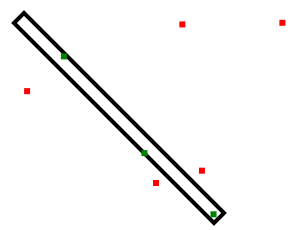
\includegraphics[scale=0.6]{pictures/touchInStroke.png}
		\caption{Test code running}
	\end{figure}

\subsection{Testing}

	\definecolor{lightgray}{gray}{0.9}

	\begin{tabular}{| p{2cm} | p{7cm} | p{3cm} |}
		\hline
		\rowcolor{lightgray}
		{\bf Test Case} & {\bf Result} & {\bf Pass/Not pass} \\ \hline

	  	FT-06 Build Power Lines &  &  \\ \hline

	  	FT-11 Collect Money &  &  \\ \hline

	  	FT-14 Win Game &  &  \\ \hline
	  	
	  	FT-16 Limited Power &  &  \\ \hline
	  	
	  	FT-17 Remove Power Cables &  &  \\ \hline
	  	
	  	FT-18 Number of Power Plants &  &  \\ \hline
	  	
	  	FT-19 Different Buildings &  &  \\ \hline

	  	FT-20 Appearance of buildings in new levels &  &  \\ \hline
	  	
	  	FT-21 More unstable power lines in new levels &  &  \\ \hline

	  	FT-22 Damaged Power Lines &  &  \\ \hline

	  	FT-24 Enter next level &  &  \\ \hline

	  	FT-25 Selected houses &  &  \\ \hline

	  	FT-26 Color of power cable &  &  \\ \hline

	  	FT-27 Power bar at power plant &  &  \\ \hline

	\end{tabular}

\subsection{Changes to the requirements}
	
	{\bf Changes on version 3 of the requirement specification:} \\
	\begin{tabular}{| p{1.5cm} | p{12cm} |}
		\hline
		\rowcolor{lightgray}
		{\bf FR} & {\bf Change} \\ \hline
		FR 4.6 & {\bf \color{green}[NEW]} The user should be able to win the game by reaching the goal in the current level. The goal is level specific. \\ \hline
		FR6.11 & {\bf \color{green}[NEW]} The user should be able to see which houses is selected when building power cables. \\ \hline
		FR6.12 & {\bf \color{green}[NEW]} The cables should change color if it is connected to a power 
		station. \\ \hline
		FR6.13 & {\bf \color{green}[NEW]} The user should be able to see how much power the powerplant have left. 
		This bar should decrease if a building is connected to the powerplant and should be 
		increase if a building is removed. The colors should be yellow whit white 
		background. \\ \hline
	\end{tabular}


\subsection{Group dynamics}

\subsection{Customer feedback}

\subsection{Sprint retrospective}
	\subsubsection*{Start doing: } 
	\subsubsection*{Stop doing: }
	\subsubsection*{Continue doing: }